A large number of migration processes have already been carried out in different scenarios outside of the company.

The migration process discussed in this document presents, however, three main peculiarities:
\begin{itemize}
    \item A huge amount of data required to migrate.
    \item The need to create custom extractors to download new data every day.
    \item A high downloading complexity.
\end{itemize}

This chapter discusses the state-of-the-art techniques used to perform migration processes, as well as various problems related to cloud migrations.
A final part will focus on different testing approaches for making sure the information stored on the cloud are identical to those already present on-premise.

\section{State of the Art}
    The amount of data Axpo required to migrate is huge and highly heterogeneous and not much information are available for such amount and complexity.
A large number of papers has been published regarding migrations to the Cloud, but few are relevant with this project.

The following publications are the most relevant regarding the migration process carried out by Axpo.

\paragraph{Architecture design}
    Some publications focus on systematic architecture design techniques, starting from the target domain \cite{bib:related_work:books:architecture}.
    The design proposed is, however, too much formal and high-level: the document focuses on understanding the needs of the company to choose which components are needed in the Cloud architecture.
    The needs are however described in a high-level notation, as shown in Figure \ref{fig:related:architecture_high_level}.
    Depending on the identified requirements, different rules are applied.
    These rules are used for specifying software architecture dependencies.
    For example, one of the rules is:
        \begin{center}
            \texttt{
                If AD HOC ANALYSIS is selected then enable INFORMATION VIRTUALIZATION on component INFORMATION MANAGEMENT SERVER.
            }
        \end{center}
    
    This design is meant for engineering a whole software architecture from scratch, not just for re-engineering a single component (in this case, the analytical back-end) while leaving the others unchanged.
    Moreover, the company was already aware of their needs, since they were the same of the on-premise structure.
    
    \begin{figure}
        \centering
        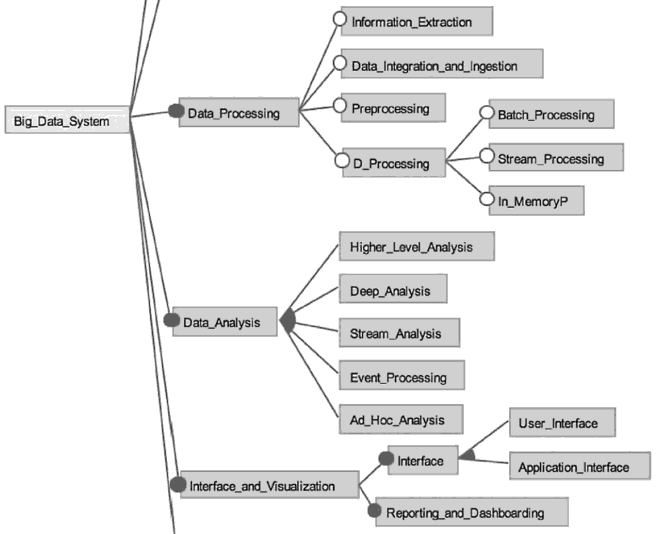
\includegraphics[width=.8\textwidth]{res/relatedwork/architecture_high_level.png}
        \caption{High-level architecture design \cite{bib:related_work:books:architecture}.}
        \label{fig:related:architecture_high_level}
    \end{figure}
    
    Issues relevant to the re-engineering process required by Axpo are also mentioned, such as the need to perform cleaning operations on data, but are not investigated or described in detail.

\paragraph{Migration process}
    Other publications focus on the re-engineering process itself, as well as some expected issues \cite{bib:related_work:books:migration}.
    The document, however, presents only a brief description of each problem, inviting readers to carry out further analyses on their own.
    The issues exposed in the publication have been also encountered during the migration process carried out by Axpo, and will be described in more details in the chapter \ref{section:etl} and in section \ref{section:dwh:remappings}.
    
    The publication also contains some remarks about potentialities offered by the Cloud, even though they are all discussed in general.
    Some of these aspects are also described in more details in this section and in chapter \ref{section:azure}.
    

\section{Moving to the Cloud}
    % why use cloud?
% https://dzone.com/articles/cloud-migration-how-and-why-business-is-moving-to

Moving workloads and data to the Cloud is becoming a reality for a very large number of companies.

According to a survey carried out in 2018 by \textit{Druva}, a cloud data management and security company, 90\% of the 170 companies interviewed have either already moved to the Cloud or intend to do so in the near future \cite{bib:related_work:migration:moving_to_cloud}.

The main drivers of these migrations are disaster recovery, ease of management, and archival.

Data in the Cloud is stored in multiple places around the world, meaning that in case of disasters no data will be lost, thanks to redundancy protocols.
The architecture itself, on the other hand, is directly managed by the Cloud provider, meaning that companies will have one less problem to worry about.

There are also other factors which make Cloud migrations more appealing, including:
\begin{itemize}
    \item Automatic scalability.
    \item Reliability.
    \item High availability.
    \item Remote access.
    \item Easier cost forecasting.
\end{itemize}


\section{Choosing the Right Process}
    % one cloud provider or many?
% switch to prod: all at once or a single component at a time?
% https://blog.newrelic.com/engineering/cloud-migration-checklist/

Before beginning a Cloud migration, it is important to take decisions with respect to several factors, which are going to influence the whole process.
The most relevant are described in what follows.

\subsection{Cloud Platform Choice}
    The first choice is whether to use a single Cloud provider or to split the application across multiple providers.
    Both choices have their own advantages and disadvantages \cite{bib:related_work:migration:10_steps}.
    
    \subsubsection{Single provider}
        Using a single Cloud provider is relatively simple.
        The development team needs to learn just one set of cloud APIs, and the application can take advantage of everything the chosen Cloud provider offers.

        The downside to this approach is vendor lock in.
        Moving the application to a different provider could require just as much effort as the original cloud migration.
        Additionally, having a single cloud provider might negatively impact the company ability to negotiate important terms, such as pricing and SLAs\footnote{
            \textit{Service Level Agreement}.
             It is the minimum level of service that a carrier will deliver to the company per agreement.
             When the service dips below that level, the company can open a repair ticket.
        }, with the cloud provider.
    
    \subsubsection{Multiple providers}
        Using multiple providers can provide several advantages, depending on the chosen model.
        
        \paragraph{Different applications on different Clouds}
            The simplest approach is to run a set of applications in one Cloud provider and a different set in another.
            This approach gives the company increased business leverage with multiple providers, as well as flexibility for where to put applications in the future.
            Each application can also be optimized for the provider on which it runs.
            
        \paragraph{Same application on multiple Clouds}
            A different approach consists of running some parts of a single application on one provider, and other parts on a different one.
            
            In this way, it is possible to effectively use the strengths of each provider.
            Let's assume, for example, that \textit{Provider A} has better AI capabilities than the other providers, while \textit{Provider B} offers cheaper and more efficient storage.
            A solution using this approach would store all data on \textit{Provider B}, and transfer only the information needed for AI models to \textit{Provider A}.
            
            There is, however, a risk tied to this approach.
            The performance of the whole application depends on the performance of each provider, meaning that the slowest provider could become a bottleneck for the whole application.
            
            Similarly, downtime of a single provider could result in the whole application not working as intended.
            
        \paragraph{Cloud-agnostic applications}
            A third possibility is building an application which can run on \textit{any} provider.
            
            There are multiple advantages, such as a higher flexibility when negotiating with providers, as well as the ability to run the same application on multiple providers at the same time.
            The latter allows more dynamic workload balancing, since it is possible to easily shift work between different providers.
            
            The downside is the inability to use each of the strengths of each provider, reducing the benefits of hosting the application in the Cloud.
            
\subsection{Migration Techniques}
    After having decided which and how many providers use, it is necessary to choose how to migrate the application to the Cloud.
    
    There are three main approaches, depending on the integration level of the application with the Cloud \cite{bib:related_work:migration:moving_to_cloud, bib:related_work:migration:10_steps}.
    
    \paragraph{Lift-and-shift}
        The simplest and fastest approach is moving the application \textit{as-is} to the cloud.
        
        With this option, however, the application cannot benefit from each of the Cloud unique services, meaning that the improvements will be reduced.
        
    \paragraph{Lift-and-refit}
        An improved version of the \textit{lift-and-shift} approach.
    
        After the application has been moved to the Cloud, some modifications are made where possible, enabling the application to leverage the strengths of the Cloud provider.
        
        The downsides are that this approach requires more time than \textit{lift-and-shift}, as well as in-depth knowledge of the application.
        Moreover, there is also the risk of increasing the complexity of the application.
        
    \paragraph{Cloud native}
        The best solution, although also the most time expensive, is to rebuild the application from scratch on the Cloud.
        
        In this way it is possible to use each of the Cloud features to the fullest, maximising both performance and readability.
        
        The downside is, however, the large amount of time needed to rewrite the whole application.
        
\subsection{Deployment}
    The last important decision is how and when to switch over the production system from the legacy on-premise solution to the new cloud version.
    
    There are two possible solutions.
    
    \paragraph{All at once}
        The switch is performed once the whole application has been successfully ported to the Cloud.
        
        All services are switched at the same moment from on-premise to Cloud.
        
    \paragraph{Incremental}
        After each part of the application has been migrated, some users move their workload to the Cloud.
        This process is then repeated until all users have successfully moved to the Cloud.
        
        For very large applications, this is the best solution, since it isn't necessary to wait for the whole migration to be complete (which could require years) before using it.

\section{Testing}
    % tests
% https://codoid.com/data-quality-checks-data-warehouse-etl/
% more tests
% https://codoid.com/etl-data-quality-testing-best-practices/

Once the source database has been migrated to the Cloud, it is important to verify the correctness of the data contained in it.
Having wrong information may cause poor business decisions, as well as other issues.

A wide array of tests can be performed on a Data Warehouse to assess the correctness of the data it contains \cite{bib:related_work:tests:tests1, bib:related_work:tests:tests2}.

Most state-of-the-art tests, however, are not suited for the energy market domain, due to the nature of the data required.

We will now analyze some of the various data quality tests widely used in the world, providing a final comparison between state-of-the-art testing techniques and the particular requirements of the energy market domain.

\subsection{Test Types}
    \paragraph{Data type coherency}
        \begin{figure}
            \centering
            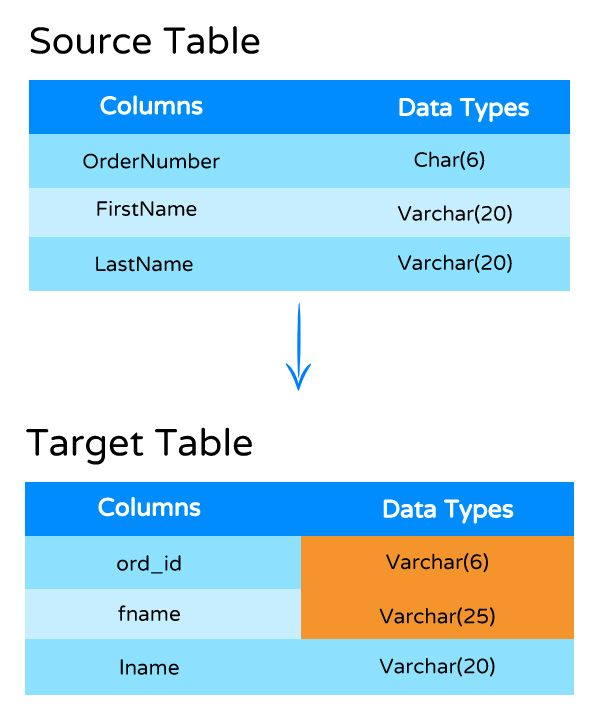
\includegraphics[width=.5\textwidth]{res/relatedwork/data_type.jpg}
            \caption{Different data types during migration.}
            \label{fig:related:tests:data_type}
        \end{figure}
        
        When performing a migration, it is important to pay attention to the format chosen for the table, not only in terms of table structure but also regarding data types used for each field.
        
        As we can see from Figure \ref{fig:related:tests:data_type}, it is possible to have mismatches between the source and destination tables.
        
        This can lead to unexpected problems.
        For example, if a \texttt{VARCHAR} field supports less characters on the destination table, the string may get truncated.
        
    \paragraph{NULL values}
        Some columns are not supposed to contain \texttt{NULL} values.
        
        It is important to make sure that any \texttt{Not NULL} constraints are respected, both by reproducing the constraint in the destination table and by specifically looking for \texttt{NULL} values.
        
        The presence of \texttt{NULL} values is often indicative of problems in the ETL process.
    
    \paragraph{Duplicate records}
        Another important test is controlling whether the destination table contains any duplicate entries where it's not supposed to, such as IDs.
        
        Having multiple instances of the same record may result in inaccurate results, leading to poor business decisions.
    
    \paragraph{Orphan records}
        \begin{figure}
            \centering
            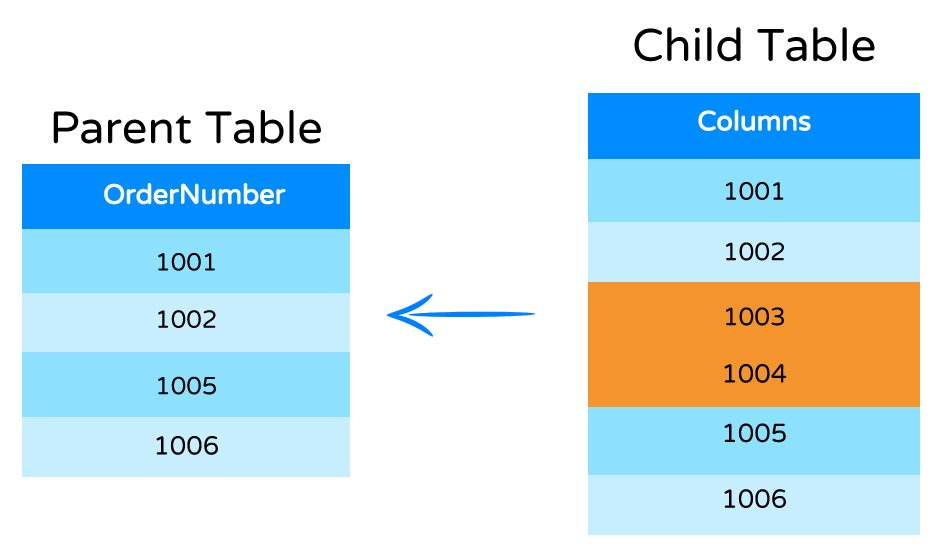
\includegraphics[width=.5\textwidth]{res/relatedwork/orphan_records.jpg}
            \caption{Orphan records.}
            \label{fig:related:tests:orphan}
        \end{figure}
        
        Orphan records are often indicative of missing data or problems in the ETL process.
        
        An orphan record can be define as an incomplete foreign key: on a child table we have an ID which doesn't appear in the parent table.
        For example, we may have billing information for a specific user, but no information about the user himself.
        
        Figure \ref{fig:related:tests:orphan} shows an example of orphan records.
        
    \paragraph{Unknown data}
        If possible, it is also a good idea to make sure values are between a reasonable range.
        
        For example, having a client over 150 years old is surely indicative of some problems.
        The same can be said for negative ages.
        
        This test can however only be applied on specific types of information: in some cases all possible values may be acceptable, such as profits or losses generated from a particular energy plant.
    
    \paragraph{Min/max validations}
        Min/max validation can assess the range of particular kinds of data.
        
        Having different ranges between the two databases can indicate either missing data (if the range is too small), or unexpected data (if the range on the cloud exceeds the local one).
    
    \paragraph{Timeliness}
        The same information may change in time.
        Downloading the same information in two different moments may give different results, if that value is updated over time.
        
        When performing a migration, it is important to pay attention to these different versions and to retrieve the correct one.
        
    
\subsection{Energy Market Domain Issues}
    Some of the tests described above are not suited for the energy market domain for a variety of reasons.
    
    \paragraph{Forecast updates}
        Energy forecasts are often updated, meaning that \textit{Timeliness} test types would fail.
        
        However, this is not a problem, since more recent versions are more accurate and are the only ones actually needed.
        
        As a consequence, these tests cannot be applied on this kind of data.
    
    \paragraph{Date ranges}
        The local database contains some data related to several years ago, which are no longer needed by any user.
        
        As such, \textit{min/max validation} tests need to be slightly tweaked.
        Instead of comparing the exact ranges, the cloud is allowed have less data, as long as these information are very old.
        
    \paragraph{Unexpected data values}
        For most values used in the energy market domain, all possible values are acceptable.
        Values outside of an ``expected'' range may indeed be indicative of unexpected market events and must as such be treated as correct.
        
        This kind of tests, as a consequence, cannot be applied on this particular process.

    

